\subsection{Ponte di Graetz} 

Verr\'a prima preso in esame il ponte di graetz come rettificatore a doppia semionda filtrato ma senza stabilizzatore a diodo zener in fig \ref{fig:bridge}.

\begin{figure}[h]
\begin{center}
	\begin{circuitikz} []
	\draw
	(0,3.05) node[transformer core](T){}
	(T.B1) to ++(0,.45) to [short,l=$\AC 7.5\, \si{\volt}_{\textrm{rms}}$] (3,3.5) to (3,3)
	(T.B2) to ++ (0,-0.45) to (3,0.5) to (3,1)
	(T.A1) to [short,l=$\AC 220\, \si{\volt}_{\textrm{rms}}$] ++ (-.5,0)
	(T.A2) to ++ (-.5,0)
	%(T.B2)+(1,0) to [open,-, l=$\AC 7.5\, \si{\volt}$] (T.B1)
	
	(2,2) to [Do] (3,3) to [Do] (4,2)
	(2,2) to [Do] (3,1) to [Do] (4,2)
	(2,2) to  (2,0.55)
	(2,0.45) to (2,0) to (5,0)
	(4,0) node[ground] {}
	(4,2) to (5,2) to [eC,l=C] (5,0)
	(5,2) to (6,2) to [R, l=$R_l$] (6,0) to (5,0) 
	(6,2) to (7,2) to [open, -*] (7,2) node[right] {$V_{out}$}
	
	;
	\end{circuitikz}
\end{center}
\caption{Ponte di Graetz con filtro capacitivo.}
\label{fig:bridge}
\end{figure}

Il condensatore elettrolitico scelto $C=220\ \si{\micro\farad}$ ha lo scopo di filtrare la doppia semionda in uscita dal ponte risultando nell'onda in fig \ref{fig:brid_cfilter}.

\begin{figure}[H]
\centering
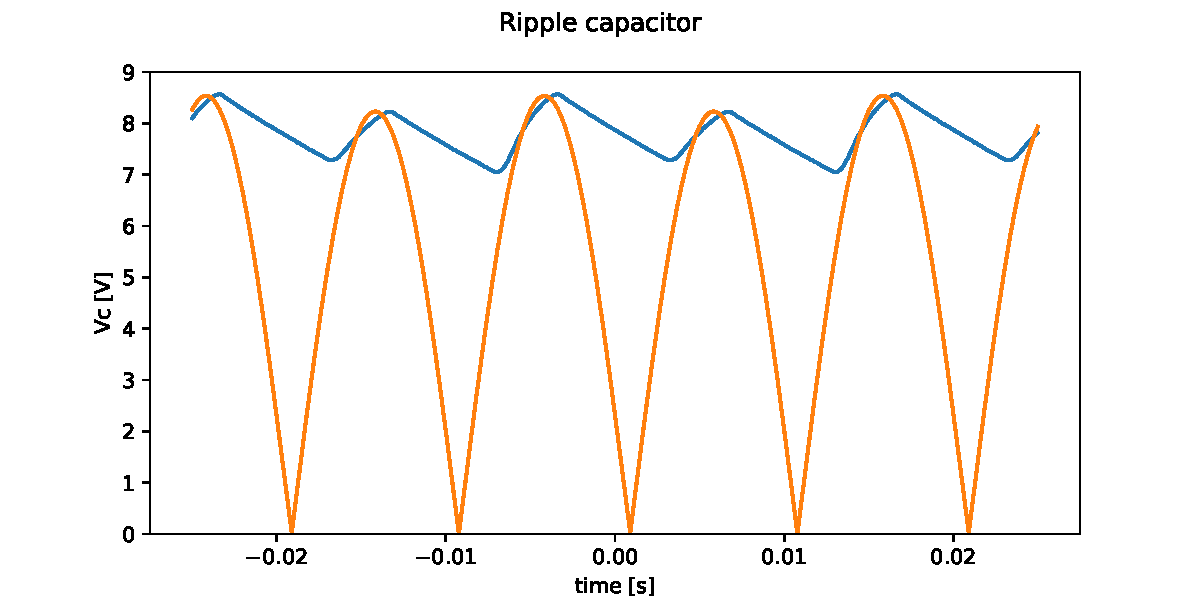
\includegraphics[width=\textwidth]{cripplefilter.pdf}
\caption{In blu la forma d'onda in uscita con il condensatore ($Rl=200\ \si{\ohm}$) ed in arancione se esso non ci fosse (quest'ultima forma d'onda \'e stata generata numericamente non potendole osservare contemporaneamente)}
\label{fig:brid_cfilter}
\end{figure}

Si pu\'o procedere a calcolare ora la massima ddp che otterrei in funzione della resistenza di carico applicata e la si confronta con i valori misurati in fig. \ref{fig:vmaxcconf}. La corrente sul carico $i_l$ \'e stata calcolata dalla $V_{out}$ misurata.

\begin{gather}
	i_{l\, max} = \frac{V_{out\, max}}{R_l} \\
	V_{out\, max} = V_{in\, max} - 2 V_d(i_{l\, max}) 
\end{gather}

\begin{figure}[h]
\centering
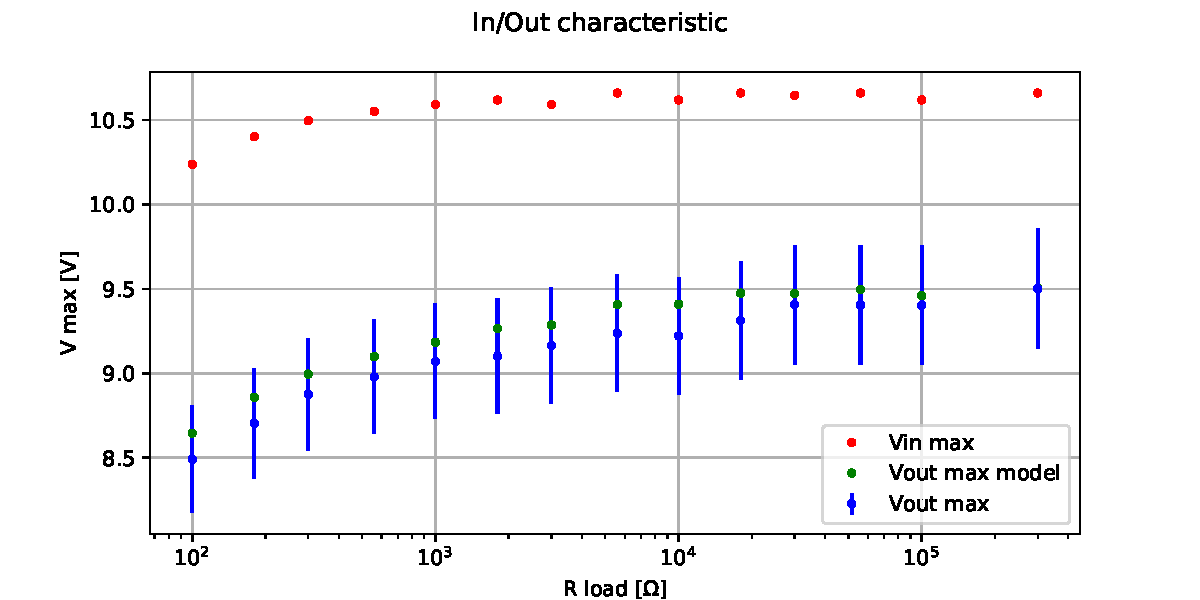
\includegraphics[width=\textwidth]{fig1.pdf}
\caption{$Vin$ misurata prima del ponte a diodi e $Vout$ misurata ai capi del carico}
\label{fig:vmaxcconf}
\end{figure}

Come si pu\'o vedere la presenza dei diodi provoca effettivamente un calo di tensione come ci si aspetta e anche l'andamento in funzione del carico \'e quello previsto.

Il ripple invece \'e mostrato in fig. \ref{fig:vppcconf}.

\begin{gather}
	V_{out\, pp} = \frac{i_{l\, max}}{2 f C}
\end{gather}

\begin{figure}[h]
\centering
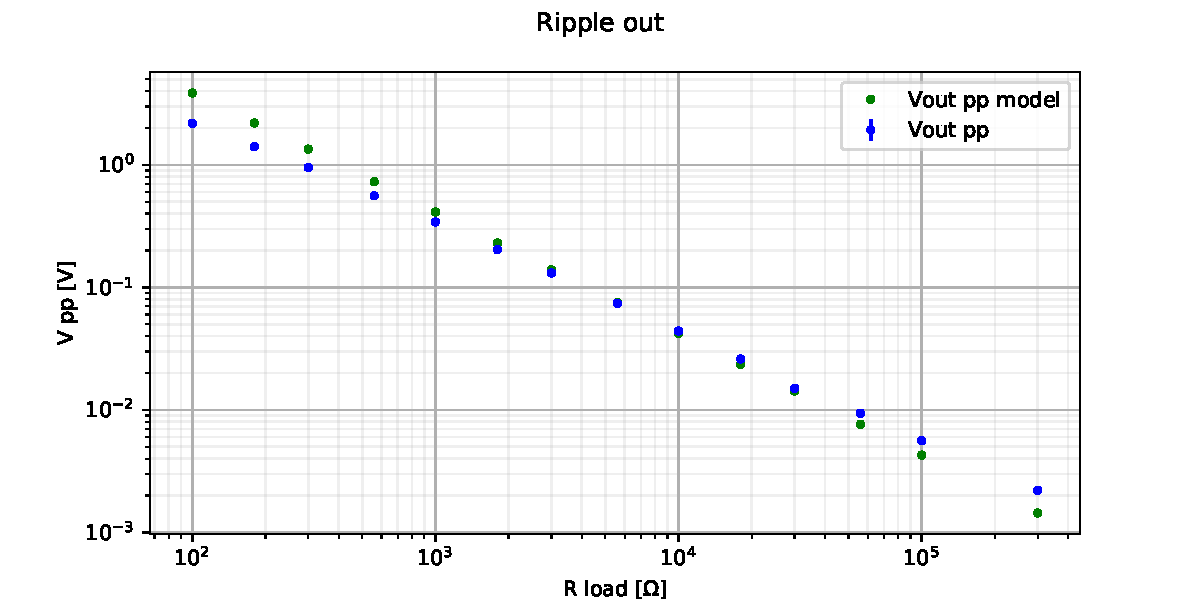
\includegraphics[width=\textwidth]{fig2.pdf}
\caption{Ripple su $Vout$ misurata ai capi del carico}
\label{fig:vppcconf}
\end{figure}

Il ripple sul condensatore segue qualitativamente l'andamento previsto e risulta del tutto compatibile per un range di carichi da $R_l=2\ \si{\kilo\ohm}$ a $R_l=30\ \si{\kilo\ohm}$.

\FloatBarrier
\newpage

Si aggiunge quindi ora il diodo zener per stabilizzare ulteriormente l'uscita secondo il circuito in figura \ref{fig:bridgez}.

\begin{figure}[h]
\begin{center}
	\begin{circuitikz} []
	\draw
	(0,3.05) node[transformer core](T){}
	(T.B1) to ++(0,.45) to [short,l=$\AC 7.5\, \si{\volt}_{\textrm{rms}}$] (3,3.5) to (3,3)
	(T.B2) to ++ (0,-0.45) to (3,0.5) to (3,1)
	(T.A1) to [short,l=$\AC 220\, \si{\volt}_{\textrm{rms}}$] ++ (-.5,0)
	(T.A2) to ++ (-.5,0)
	%(T.B2)+(1,0) to [open,-, l=$\AC 7.5\, \si{\volt}$] (T.B1)
	
	(2,2) to [Do] (3,3) to [Do] (4,2)
	(2,2) to [Do] (3,1) to [Do] (4,2)
	(2,2) to  (2,0.55)
	(2,0.45) to (2,0) to (5,0)
	(4,0) node[ground] {}
	(4,2) to (5,2) to [eC,l=C] (5,0)
	(5,2) to [R,l=R,i>_=$i_R$] (7,2) to [zzDo,invert,i>_=$i_z$] (7,0)
	(7,2) to (8,2) to [R, l=$R_l$,i>_=$i_l$] (8,0) to (5,0) 
	(8,2) to (9,2) to [open, -*] (9,2) node[right] {$V_{out}$}
	(5,2) to (5,3) to (9,3) to [open, -*] (9,3) node[right] {$V_c$}
	
	;
	\end{circuitikz}
\end{center}
\caption{Ponte di Graetz con filtro capacitivo e diodo zener.}
\label{fig:bridgez}
\end{figure}

In questa configurazione il diodo svolge la funzione di diminuire il ripple (fig. \ref{fig:ripplecomp}) che si era visto con solamente il condensatore al costo di dissipare potenza nella resistenza $R$ e nello zener.

\begin{figure}[h]
\centering
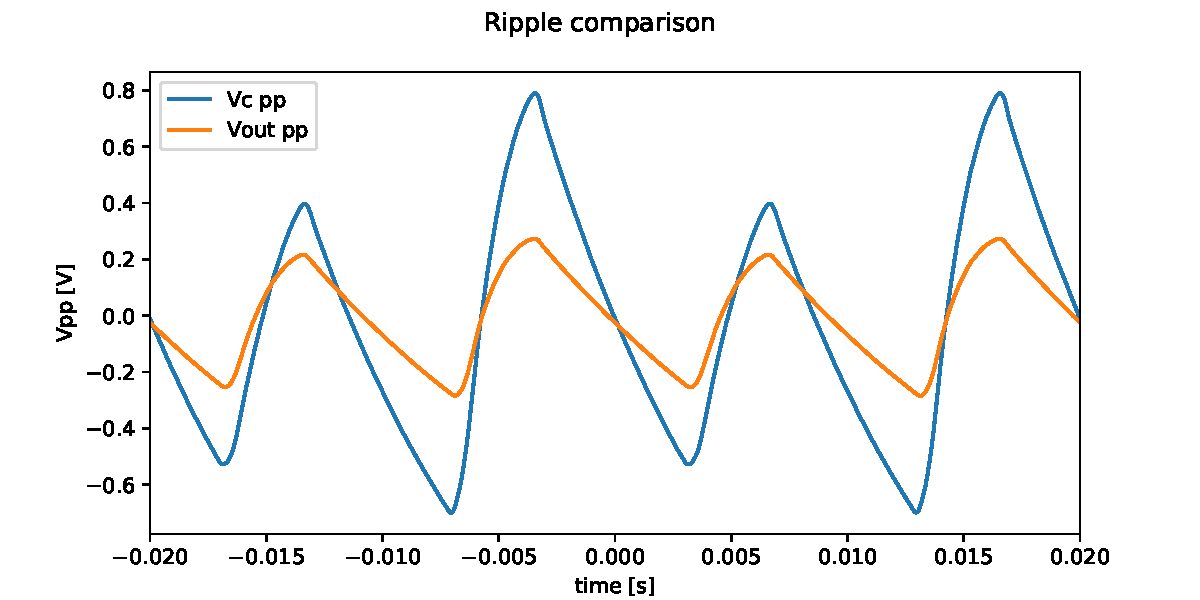
\includegraphics[width=\textwidth]{ripplecomp.pdf}
\caption{Confronto ripple con $R_l = 200 \ \si{\ohm}$.}
\label{fig:ripplecomp}
\end{figure}

Chiamata $i_z(V_z)$ la caratteristica tensione-corrente dello zener ed utilizzando la $V_{out}$ misurata per il calcolo di $i_l$ e $i_z$ si pu\'o definire:

\begin{gather}
	i_{l\, max} = \frac{V_{out\, max}}{R_l} \\
	i_{z\, max} = i_z(V_{out\, max}) \\
	i_{R\, max} = i_{z\, max} + i_{out\, max} \\
	V_{out\, max} = V_{c\, max} - i_{R\, max} R
\end{gather}


Come si pu\'o vedere la presenza dello stadio ulteriore di filtraggio diminuisce l'output del circuito e il confronto \'e mostrato in figura \ref{fig:vdiod}.

\begin{figure}[H]
\centering
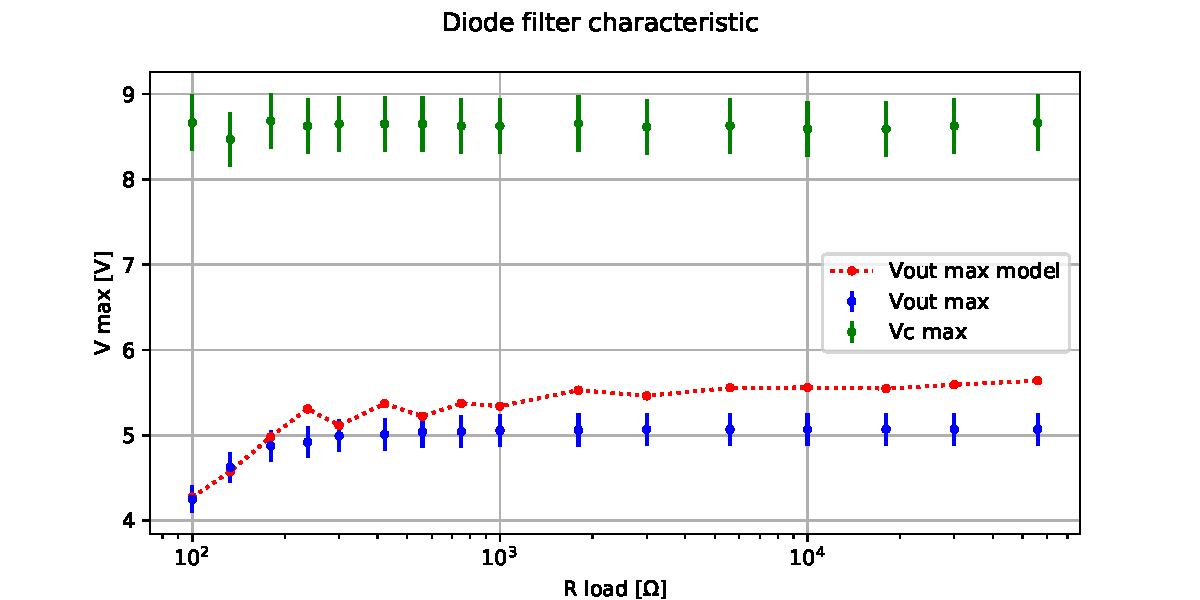
\includegraphics[width=\textwidth]{fig4.pdf}
\caption{$V_{out\, max}$ in funzione del carico}
\label{fig:vdiod}
\end{figure}

Considerata $r_z(i_z)$ la resistenza dinamica del diodo, il ripple viene stimato in questo modo:

\begin{gather}
	V_{c\, pp} = \frac{i_{R\, max}}{2fC} \\
	V_{out\, pp} = V_{c\, pp} \frac{r_z}{r_z+R(1+\frac{r_z}{R_l})}
\end{gather}

E quindi confrontato in figura \ref{fig:vdiodpp} da cui si vede che per valori di carico inferiore al kiloOhm il ripple aumenta fino al $15\%$ di $V_{out\, max}$ (corrispondente a $R_l=100\ \si{\ohm}$). Questo \'e dovuto al fatto che una resistenza $R_l$ minore aumenta la corrente che scorre nella resistenza $R$ che a sua volta diminuisce la tensione in uscita facendo lavorare il diodo su di una retta di carico passante per la parte non ideale della caratteristica tensione-corrente del diodo Zener il quale per correnti piccole soggette a fluttuazioni provoca una fluttuazione della tensione ai capi relativamente maggiore rispetto a correnti mediamente pi\'u intense. Per migliorare le prestazioni per questo range di carichi si suggerisce di diminuire la resistenza $R$ prestando attenzione al fatto che questo provoca una dissipazione di potenza ancora maggiore da parte di $R$ e del diodo nel caso di circuito aperto.

\begin{figure}[h]
\centering
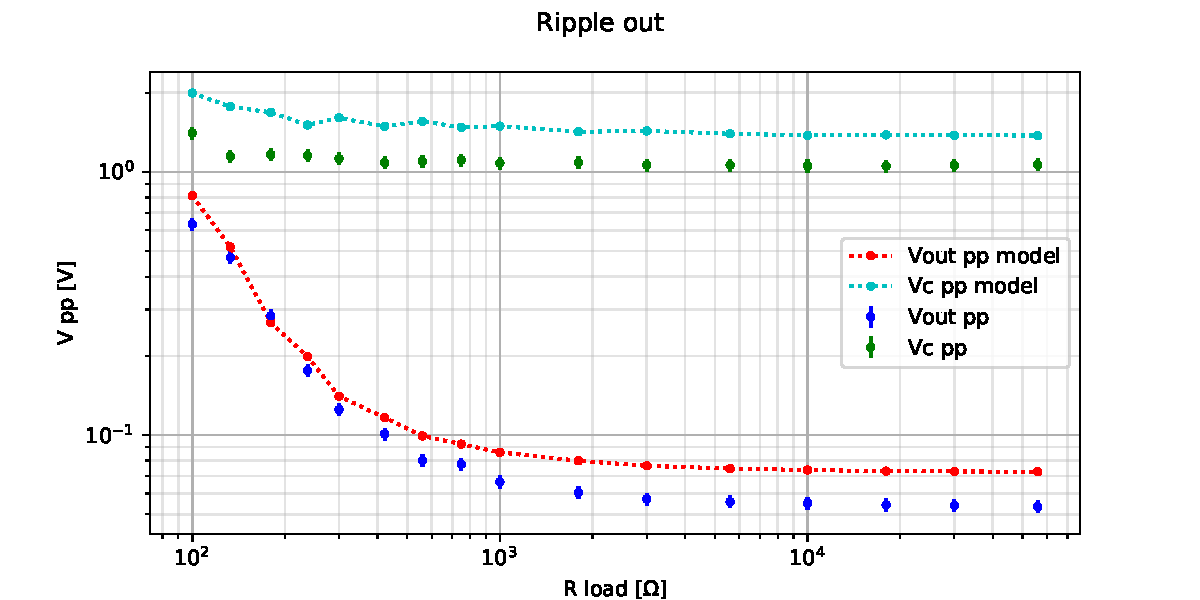
\includegraphics[width=\textwidth]{fig5.pdf}
\caption{Ripple in funzione del carico.}
\label{fig:vdiodpp}
\end{figure}

Si pu\'o inoltre esaminare la resistenza in uscita $R_{out}$ mostrata dal circuito, fig. \ref{fig:rout}.

\begin{gather}
	R_{out} = \frac{V_{out\, c.a.} - V_{out}}{i_{out}}
\end{gather}

\begin{figure}[h]
\centering
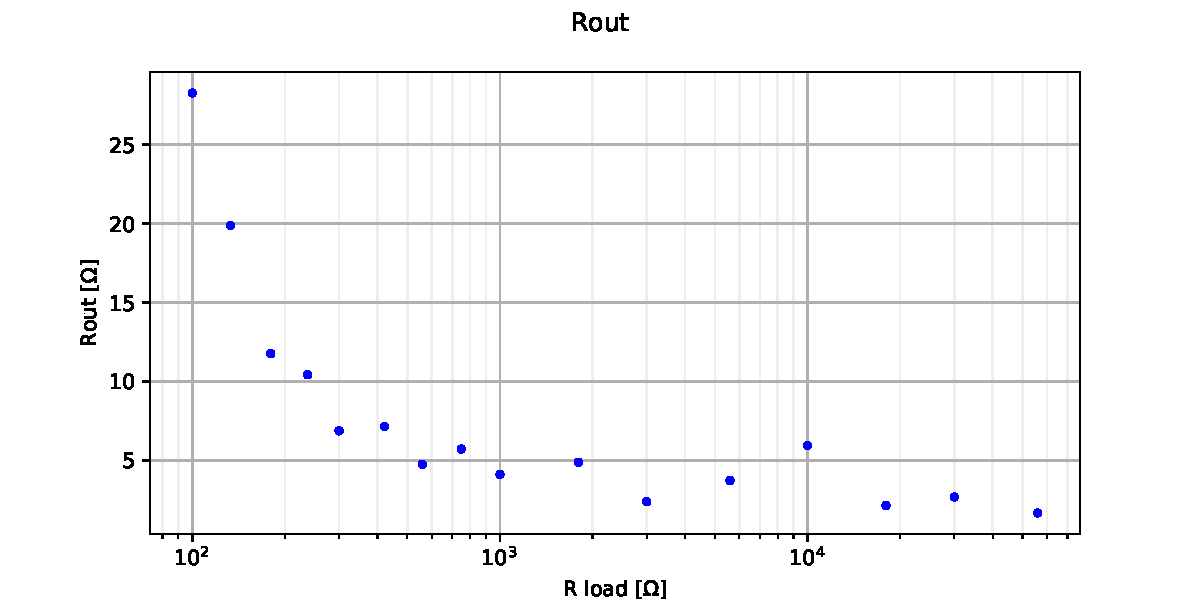
\includegraphics[width=\textwidth]{fig6.pdf}
\caption{$R_{out}$ in funzione del carico.}
\label{fig:rout}
\end{figure}

\FloatBarrier

Il costo in termini di potenza dissipata per diminuire il ripple risulta:

\begin{gather}
	P_d = i_R^2 R + i_z V_{out}
\end{gather}

Questa potenza persa causa una diminuzione dell'efficienza del circuito al diminuire della corrente assorbita dal carico come si pu\'o vedere in figura \ref{fig:eff}.

\begin{figure}[H]
\centering
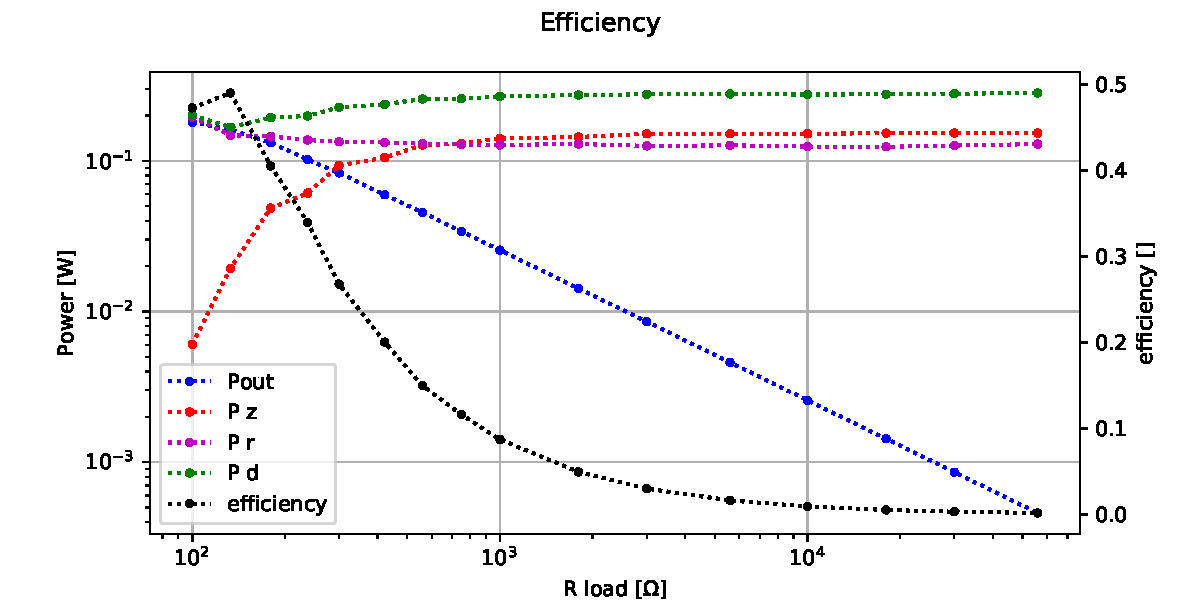
\includegraphics[width=\textwidth]{fig7.pdf}
\caption{Efficienza: $P_{out}$ potenza sul carico, $P_{z}$ potenza dissipata dal diodo zener, $P_{r}$ potenza dissipata dalla resistenza $R$ e $P_{d}$ totale della potenza persa nel filtering.}
\label{fig:eff}
\end{figure}









